\documentclass[main.tex]{subfiles}
\begin{document}



\section{Continue functie van $\mathbb{R}^{p}$ naar $\mathbb{R}^{q}$ }
\label{sec:continue-functie-van}

\begin{de}
  Zij $f:\ A \subseteq \mathbb{R}^{p} \rightarrow \mathbb{R}^{q}$ een functie en $a$ een element van $A$, dan noemen we $f$ \term{continu} in $a$ als het volgende geldt:
  \[ \forall \epsilon \in \mathbb{R}_{0}^{+}, \exists \delta \in \mathbb{R}_{0}^{+}, \forall x \in A:\ \|x-a\| < \delta \Rightarrow \|f(x)-f(a)\| < \epsilon \]
\end{de}

\begin{de}
  We noemen $f$ \term{continu} op $A$ als $f$ continu is in elke $a\in A$.
  \[ \forall a\in A, \forall \epsilon \in \mathbb{R}_{0}^{+}, \exists \delta \in \mathbb{R}_{0}^{+}, \forall x \in A:\ \|x-a\| < \delta \Rightarrow \|f(x)-f(a)\| < \epsilon \]
\end{de}

\begin{pr}
  \label{pr:in-rp-continu-asa-limiet-van-elke-rij}
  Zij $f:\ A \subseteq \mathbb{R}^{p} \rightarrow \mathbb{R}^{q}$ een functie en $a$ een element van $A$, dan is $f$ continu in $a$ als en slechts als er voor elke rij $(x_{n})_{n}$ in $A$ die naar $a$ convergeert geldt dat $(f(x_{n}))_{n}$ naar $f(a)$ convergeert.
\extra{bewijs}
\end{pr}

\begin{pr}
  Een functie $f:\ A \subseteq \mathbb{R}^{p} \rightarrow \mathbb{R}^{q}$ is continu in $a\in A$ als en slechts als alle componentsfuncties $f_{i}:\ A \subseteq \mathbb{R}^{p} \rightarrow \mathbb{R}$ continu zijn in $a$.

  \begin{proof}
    Inderdaad\stref{st:in-rp-convergeert-asa-componenten-convergeren}\prref{pr:in-rp-continu-asa-limiet-van-elke-rij}
  \end{proof}
\end{pr}

\begin{pr}
  Zij $f:\ A \subseteq \mathbb{R}^{p} \rightarrow \mathbb{R}^{q}$ een functie en $a$ een element van $A$, dan is $f$ continu in $a$ als en slechts als er voor elke open deelverzameling $V$ van $\mathbb{R}^{q}$ geldt dat $f^{-1}(V)$ relatief open is in $A$.
\extra{bewijs}
\end{pr}

\begin{de}
  Beschouw een functie $f:\ A \subseteq \mathbb{R}^{p} \rightarrow B \subseteq \mathbb{R}^{q}$ en een $a\in A$, dan definieren we de \term{partiele functies} $f_{i}$ van $f$ in $a$ als volgt:
  \[ f_{i}:\ A_{i} \rightarrow B:\ t \mapsto f_{i}(t) = f(a_{1},\dotsc,a_{i-1},t,a_{i+1},\dotsc,a_{p}) \]
\end{de}

\begin{pr}
  Als $f$ continu is in $a$, dan zijn alle parti\"ele functies $f_{i}$ continu in $a_{i}$.

  \begin{proof}
    Noteer $A_{i}$ als volgt:
    \[ A_{i} = \{ t\in \mathbb{R} \mid (a_{1},\dotsc,a_{i-1},t,a_{i+1},\dotsc,a_{p}) \in A \} \]
    Kies willekeurig een $i\in \{1,\dotsc,p\}$ en een willekeurige rij $(t_{n})_{n}$ in $A_{i}$ die naar $a_{i}$ convergeert.
    Noem bovendien $(x_{n})_{n} = (a_{1},\dotsc,a_{i-1},t_{n},a_{i+1},\dotsc,a_{p})_{n}$, dan is $(x_{n})_{n}$ een rij in $A$ die naar $a$ convergeert.\prref{pr:in-rp-continu-asa-limiet-van-elke-rij}
    Nu convergeert bijgevolg $f_{i}(t_{n}) = f(x_{n})$ naar $f(a) = f_{i}(a_{i})$.
\clarify{meer uitleg?}
  \end{proof}
\end{pr}

\begin{tvb}
  Het omgekeerde van bovenstaande stelling geldt niet.
  
  \begin{proof}
    Beschouw de functie $f$ als volgt:
    \[ 
    f:\ \mathbb{R}^{2} \rightarrow \mathbb{R}:\ (x_{1},x_{2}) \mapsto 
    \begin{cases}
      \frac{x_{1}x_{2}}{x_{1}^{2}+x_{2}^{2}} & \text{ als } (x_{1},x_{2}) \neq (0,0)\\
      0 & \text{ als } (x_{1},x_{2}) = (0,0)
    \end{cases}
    \]
    \begin{figure}[H]
      \centering
      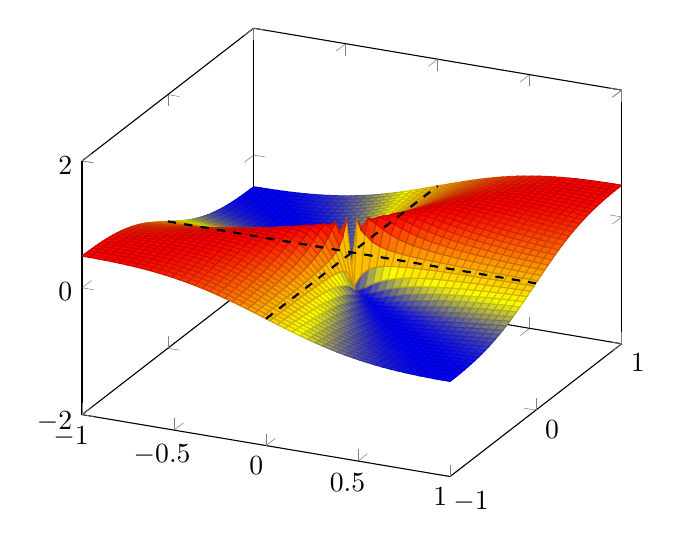
\begin{tikzpicture}
        \begin{axis}[samples=50,restrict z to domain=-50:50,zmax=2,zmin=-2]
          \addplot3[surf, domain=-1:1,y domain=-1:1, z buffer=sort] {(x*y)/(x^2+y^2)};
          \addplot3[mark=,thick,dashed] coordinates {(-1,0,0) (1,0,0)};
          \addplot3[mark=,thick,dashed] coordinates {(0,-1,0) (0,1,0)};
        \end{axis}
      \end{tikzpicture}
      \caption{$f$}
    \end{figure}
    Kies $a=(0,0)$. Hier zijn de parti\"ele functies van $f$ in $a$ identiek nul en dus zeker continu in $0$.
    $f$ is niettemin niet continu in $a$.\waarom
  \end{proof}
\end{tvb}

\begin{pr}
  Zij $f:\ A \subseteq \mathbb{R}^{p} \rightarrow \mathbb{R}^{q}$ een functie die continu is in $a\in A$ en $\lambda$ een element van $\mathbb{R}$, dan is $\lambda f$ continu in $a$.
  \extra{bewijs}
\end{pr}

\begin{pr}
  Zij $f,g:\ A \subseteq \mathbb{R}^{p} \rightarrow \mathbb{R}^{q}$ twee functies die continu zijn in $a\in A$, dan is $f+g$ continu in $a$.
  \extra{bewijs}
\end{pr}

\begin{pr}
  Voor $q=1$:
  Zij $f,g:\ A \subseteq \mathbb{R}^{p} \rightarrow \mathbb{R}^{q}$ twee functies die continu zijn in $a \in A$, dan is $fg$ continu in $a$.
  \extra{bewijs}
\end{pr}

\begin{pr}
  Voor $q=1$:
  Zij $f,g:\ A \subseteq \mathbb{R}^{p} \rightarrow \mathbb{R}^{q}$ twee functies die continu zijn in $a \in A$, dan is $\nicefrac{f}{g}$ continu in $a$ als $g(a)$ niet nul is.
  \[ \nicefrac{f}{g}:\ A \setminus \{b \in A \mid g(b) = 0 \} \Rightarrow \mathbb{R}:\ x \mapsto \frac{f(x)}{g(x)} \]
  \extra{bewijs}
\end{pr}

\begin{pr}
  Zij $f:\ A \subseteq \mathbb{R}^{p} \rightarrow B \subseteq \mathbb{R}^{q}$ en $f:\ B \subseteq \mathbb{R}^{q} \rightarrow \rightarrow \mathbb{R}^{m}$ twee functies.
  Als $f$ continu is in $a\in A$ en $g$ continu in $f(a)$, dan is $g\circ f$ continu in $a$.
\extra{bewijs}
\end{pr}

\begin{pr}
  Zij $A$ een gesloten begrensd deel van $\mathbb{R}^{p}$ en zij $f:\ A \rightarrow \mathbb{R}^{q}$ een continue injectieve functie, dan is $f^{-1}:\ f(A) \rightarrow A$ ook continu.
\extra{bewijs}
\end{pr}

\begin{st}
  Beschouw een continue functie $f:\ A \subseteq \mathbb{R}^{p} \rightarrow \mathbb{R}$ , met $A$ gesloten en begrensd, dan is $f$ begrensd en bereikt $f$ op $A$ haar minimale en maximale waarde.
  Er bestaan dus een $c$ en $d$ als volgt:
  \[ f(c) = \sup\{ f(x) \mid x\in A\} \quad \text{ en } \quad f(d) = \inf\{f(x) \mid x\in A\} \]
\extra{bewijs}
\end{st}

\begin{st}
  Beschouw een continue functie $f:\ A \subseteq \mathbb{R}^{p} \rightarrow \mathbb{R}^{q}$, met $A$ gesloten en begrensd, dan is $f(A)$ ook gesloten en begrensd.

  \begin{proof}
    Bewijs uit het ongerijmde: Stel dat $f(A)$ niet begrensd, of niet gesloten is.
    \begin{itemize}
    \item Stel dat $f(A)$ niet begrensd is.\\
      We kunnen dan voor elke $n\in mathbb{N}$ een $x_{n} \in A$ kiezen met $\|f(x_{n})\| > n$ om een rij $(x_{n})_{n}$ in $A$ te construeren.
      Omdat $A$ gesloten en begrensd is, kunnen we een deelrij $(x_{n_{k}})_{k}$ nemen die convergeert naar een $x\in A$.\stref{st:in-rp-gesloten-en-begrensd-itv-rijen}
      Omdat $f$ continu is, moet $(f(x_{n_{k}}))_{k}$ naar $f(x)$ convergeren.\prref{pr:in-rp-continu-asa-limiet-van-elke-rij}
      Omdat $(f(x_{n_{k}}))_{k}$ convergent is, moet de rij begrensd zijn\stref{st:in-rp-convergent-dan-begrensd}, maar dit in strijd met de contructie ($\forall n\in \mathbb{N}: \|f(x_{n})\| > n$) van $(x_{n_{k}})_{k}$.
      Contradictie.
    \item Stel dat $f(A)$ niet gesloten is.\\
      Er bestaat dan een rij $(y_{n})_{n}$ in $F(A)$ die convergeent naar een $y\in \mathbb{R}^{q}\setminus f(A)$.\prref{pr:in-rp-continu-asa-limiet-van-elke-rij}
      Kies nu $x_{n} \in A$ zodat $f(x_{n}) = y_{n}$, dan verkrijgen we een rij $(x_{n})_{n}$ in $A$ die, omdat $A$ gesloten en begrensd is, een convergente deelrij $(x_{n_{k}})_{k}$ heeft met limiet in $A$.\stref{st:in-rp-gesloten-en-begrensd-itv-rijen}
      Omdat $f$ continu is, zal $(y_{n_{k}})_{k}$ naar $f(x)$ convergeren.\prref{pr:in-rp-continu-asa-limiet-van-elke-rij}
      Omdat $(y_{n_{k}})_{k}$ een deelrij is van een convergente rij $(y_{n})_{n}$ moet $(y_{n_{k}})_{k}$ dezelfde limiet $y$ hebben.\stref{st:in-rp-deelrij-zelfde-limiet}
      Dit kan niet omdat $f(x)$ in $f(A)$ zit maar $y$ niet.
      Contradictie.
    \end{itemize}
  \end{proof}
\end{st}


\subsection{Uniformu continu\"iteit}
\label{sec:unif-cont}

\begin{de}
  We noemen een functie $f:\ A \subseteq \mathbb{R}^{p} \rightarrow \mathbb{R}^{q}$ \term{uniform continu} op $A$ als en slechts als het volgende geldt:
  \[ \forall \epsilon \in \mathbb{R}_{0}^{+}, \exists \delta \in \mathbb{R}_{0}^{+}, \forall x,y \in A:\ \|x-y\| < \delta \Rightarrow \|f(x)-f(y)\| < \epsilon \]
\end{de}

\begin{st}
  Zij $f:\ A \subseteq \mathbb{R}^{p} \rightarrow \mathbb{R}^{q}$ een continue functie op een een gesloten, begrensd deel $A$ van $\mathbb{R}^{p}$, dan is $f$ uniform continu.
\extra{bewijs}
\end{st}

\begin{st}
  Een lineaire afbeelding $T:\ \mathbb{R}^{p}\rightarrow \mathbb{R}^{q}$ is uniform continu.

  \begin{proof}
    Zij $T:\ \mathbb{R}^{p}\rightarrow \mathbb{R}^{q}$ een lineaire afbeelding en $\beta = \{e_{1},e_{2},\dotsc,e_{p}\}$ een orthonormale basis van $\mathbb{R}^{p}$.
    Noem $M = \sup\{\|T(e)\| \mid e \in \beta \}$.
    Beschouw nu de volgende afschatting van $\|T(x)\|$ voor elke $x\in \mathbb{R}^{p}$.
    Merk op dat we $x$ kunnen schrijven in termen van de basis $\beta$, zeg als $x = \sum_{i=1}^{p}\lambda_{i}e_{i}$.
    \[
    \|T(x)\|
    = \left\| \sum_{i=1}^{p}\lambda_{i}T(e_{i}) \right\|
    \le \sum_{i=1}^{p} |\lambda_{i}|\|T(e_{i})\|
    \le \sum_{i=1}^{p} M |\lambda_{i}|
    \le M \sqrt{p} \|x\|
    \]
    \clarify{die laatste stap is niet echt rigoreus, enkel intu\"itief.}
    Kies nu een $\epsilon \in \mathbb{R}_{0}^{+}$ en kies $\delta = \frac{\epsilon}{M\sqrt{p}}$.
    Kies bovendien twee elementen $x,y\in \mathbb{R}^{p}$ die dichter dan $\delta$ bij elkaar liggen.
    \[ \|T(x)-T(y)\| = \|T(x-y)\| \le M\sqrt{p}\|x-y\| < \frac{M \sqrt{p}\epsilon}{M\sqrt{p}} = \epsilon \]
  \end{proof}
\feed
\end{st}


\subsection{Middelwaardestellingen}

\begin{de}
  Zij $\mathbb{R},V,+$ een reele vectorruimt, dan noemen we een deelverzameling $A$ van $V$ \term{convex} als en slechts als het volgende geldt:
  \[ \forall a,b \in A, \forall \lambda \in \interval{0}{1}:\ (1-\lambda)a+\lambda b \in A \]
\end{de}

\begin{pr}
  Beschouw een continue functie $f:\ A \subseteq \mathbb{R}^{p} \rightarrow \mathbb{R}$ met $A$ convex.
  Zij $a,b\in A$ en kies een $y\in \mathbb{R}$ tussen $f(a)$ en $f(b)$, dan bestaat er minstens \'e\'e $c\in A$ op het lijnstuk dat $a$ en $b$ verbindt zodat $f(c) = y$ geldt of dus een $\lambda \in \interval{0}{1}$ als volgt:
  \[ f((1-\lambda)a+\lambda b) = y \]

  \begin{proof}
    Merk op dat het enkel zinvol is om over $f$ op het lijnstuk tussen twee punten $a$ en $b$ uit $A$ te praten als $A$ convex is.
    Beschouw de continue functie $g$ als volgt:
    \[ g:\ \interval{0}{1} \rightarrow \mathbb{R}:\ \lambda \mapsto g(\lambda) = f((1-\lambda)a+\lambda b) \]
    Merk op dat $g(0)$ gelijk is aan $f(a)$ en $g(1)$ gelijk aan $f(b)$.
    $y$ ligt dus tussen $g(0)$ en $g(1)$.
    We passen de tussenwaardestelling toe op $g$ en het interval $\interval{0}{1}$ om een $\lambda\in \interval{0}{1}$ te vinden met beeld $y$ onder $g$.\stref{st:tussenwaardestelling}
    $y$ is dus het beeld van een $c$ ,op het lijnstuk tussen $a$ en $b$, onder $f$.
  \end{proof}
\end{pr}


\subsection{Rijen van continue functies}
\label{sec:rijen-van-continue}

\begin{de}
  Beschouw een rij $(f_{n})_{n}$ van functies $f_{n}:\ A \rightarrow \mathbb{R}^{q}$, dan zeggen we dat $(f_{n})_{n}$ \term{puntsgewijs convergeert} op $A$ naar een functie $f:\ A \rightarrow \mathbb{R}^{q}$ als het volgende geldt:
  \[ \forall x\in A, \forall \epsilon \in \mathbb{R}_{0}^{+}, \exists n_{0} \in \mathbb{N}, \forall n \in \mathbb{N}:\ n \ge n_{0} \Rightarrow \|f_{n}(x) -f(x)\| < \epsilon \]
\end{de}

\begin{de}
  Beschouw een rij $(f_{n})_{n}$ van functies $f_{n}:\ A \rightarrow \mathbb{R}^{q}$, dan zeggen we dat $(f_{n})_{n}$ \term{uniform convergeert} op $A$ naar een functie $f:\ A \rightarrow \mathbb{R}^{q}$ als het volgende geldt:
  \[ \forall \epsilon \in \mathbb{R}_{0}^{+}, \exists n_{0} \in \mathbb{N}, \forall x\in A, \forall n \in \mathbb{N}:\ n \ge n_{0} \Rightarrow \|f_{n}(x) -f(x)\| < \epsilon \]
\end{de}

\begin{st}
  Beschouw een rij $(f_{n})_{n}$ van functies $f_{n}:\ A \subseteq \mathbb{R}^{p} \rightarrow \mathbb{R}^{q}$ die uniform convergeert naar een functie $f:\ A \rightarrow \mathbb{R}^{q}$, dan geldt:
  \begin{itemize}
  \item $f$ is continu in $a$ als alle $f_n$ continu zijn in $a$.
  \item $f$ is uniforum continu op $A$ als alle $f_n$ uniform continu zijn op $A$.
  \end{itemize}
\extra{bewijs}
\end{st}


\end{document}

%%% Local Variables:
%%% mode: latex
%%% TeX-master: t
%%% End:
